\section{Proof Discharge Algorithm through Examples}
\label{sec:syn-examples}
This section demonstrates our proof discharge algorithm through example programs
that construct and traverse a linked list respectively. Our equivalence checker has the property
that it is safe to return false (i.e. disproven) for all proof obligations. Keeping this in mind,
our proof discharge algorithm is designed to be {\em sound} i.e. (a) whenever it evaluates a proof obligation
to true (i.e. proven), the actual proof obligation must also be proven and (b) whenever it returns
false with a set of counterexamples, the counterexamples must falsify the actual proof obligation.
However, it is possible for our proof discharge algorithm to return false (without a counterexample)
even if the actual proof obligation is true.
Our equivalence checking algorithm also ensures that, for an invariant
$\phi_s=({\tt \phi^{1}_s \land \phi^{2}_s \land ... \land \phi^{k}_s})$,
at any node $s$ of a product-CFG,
if a \recursiveRelation{} appears in $\phi_s$, it
must be one of $\phi^{1}_s$, $\phi^{2}_s$, ..., or $\phi^{k}_s$. We call
this the {\em conjunctive \recursiveRelation{}} property of an invariant $\phi_s$.

A proof obligation
$\hoareTriple{\phi_s}{e}{\phi_d}$, where $e=(\rho_S,\rho_C)$,
gets lowered using
${\tt WP}_{e}(\phi_d)$ (as shown in \cref{eqn:firstOrderFormula}) to a first-order logic formula of the following form:
\vspace{-5px}
\begin{equation}
\label{eqn:proofObligationShape}
(\eta^{l}_1 \land \eta^{l}_2 \land ... \land \eta^{l}_m) \Rightarrow (\eta^{r}_1 \land \eta^{r}_2 \land ... \land \eta^{r}_n)
\vspace{-5px}
\end{equation}
% In this formula,
% the {\tt LHS} and {\tt RHS} are
% written as conjunctions of $\eta^{l}_i$ and $\eta^{r}_j$ respectively (for $1\leq i\leq m$, $1\leq j\leq n$).
% Each $\eta^{r}_j$ relation is obtained from
% ${\tt WP}_{e}(\phi^{j}_d)$, where $\phi_d=({\tt \phi^{1}_d \land \phi^{2}_d \land ... \land \phi^{n}_d})$.
Thus, due to the conjunctive \recursiveRelation{} property of $\phi_s$ and $\phi_d$, any
\recursiveRelation{} in \cref{eqn:proofObligationShape} must appear as
one of $\eta^{l}_i$ or $\eta^{r}_j$.
To simplify proof obligation discharge,
we break a first-order logic proof obligation $P$ of the form in \cref{eqn:proofObligationShape}
into multiple smaller proof obligations
of the form
$P_j:(\lhs{} \Rightarrow{\tt \eta^{r}_j})$, for $j=1..n$. Each proof obligation
$P_j$ is then discharged separately.  We call this conversion from
a bigger query to multiple smaller queries, {\em \rhs{}-breaking}.

%We say that two relations $\eta_1$ and $\eta_2$ {\em interfere}, written
%$\eta_1 \interfere{} \eta_2$,
%iff the intersection
%of the sets of free variables mentioned in $\eta_1$ and $\eta_2$
%is non-empty.  For example, $a\indEq{}b$ and $c\indEq{}d$
%do not interfere, but $a\indEq{}b$ and $c\indEq{}{\tt LCons}(0,b)$ interfere.
%
%In a proof obligation of the form in \cref{eqn:proofObligationShape},
%two relations $\eta_1$ and $\eta_2$ {\em transitively interfere} iff
%there exists a relation $\eta_3$ in the proof
%obligation such that $\eta_1\interfere{}\eta_3$ and $\eta_3\interfere{}\eta_2$.
%This notion of transitive interference can be lifted
%to Hoare triples: in a proof obligation $\{\phi_s\}(e)\{\phi_d\}$,
%where $\phi_{s}=\phi^{1}_s\land...\phi^{k}_{s}$ and $\phi_{d}=\phi^{1}_d\land...\phi^{n}_{d}$,
%an {\tt LHS} conjunctive clause $\phi^{i}_s$ transitively
%interferes with an {\tt RHS} conjunctive clause $\phi^{j}_d$ iff
%$\phi^{i}_s$
%transitively interferes with ${\tt WP}_{e}(\phi^{j}_d)$ in
%the lowered first-order logic formula.

%We provide a sound (but imprecise) proof discharge
%algorithm that converts
%a proof obligation generated by our equivalence
%checker into a series of SMT queries.
%Our
%algorithm begins
%by categorizing a proof obligation
%into three categories, and each
%category is discussed separately
%in subsequent sections.  These categories are created
%based on an iterative unrolling and unification
%procedure, which we describe next.
%We use an unroll parameter $k$ for
%our categorization.
\subsection[Categorization of Proof Obligations]{Categorization of Proof Obligations based on \\Decomposition of Recursive Relations}
\label{sec:syn-cat-decomp}
Before diving into the proof discharge algorithm, we start with a key procedure in our proof discharge algorithm called `decomposition of \recursiveRelations{}'.
\vspace{-5px}
\begin{equation}
\label{eqn:specDeconstruct}
U_S: l = \sumIf{\sumIs{l}{LNil}} \  \sumThen{\cons{LNil}} \  \sumElse{\cons{LCons}(\prodAccess{l}{val}, \prodAccess{l}{next})}
\vspace{-5px}
\end{equation}
Firstly, an expression $e$ whose top-level operator is a lifting constructor, (e.g., \lifted{list}{\mem{}}{lnode}{\cv{l}}), is called a {\em lifted expression}.
A \recursiveRelation{} of the form $l_1 \indEq{} l_2$ can be {\em decomposed} into an
equivalent set of {\em decomposition clauses}, each of the form $(P\! \rightarrow\! A\! =\! B)$ or $(P\! \rightarrow\! A\! \indEq{}\! B)$.
The primary algorithm behind decomposition is an iterative unification and rewriting procedure under a set of rewriting rules $E$.
$E$ allows rewriting of lifted expressions by their corresponding definitions (e.g., \cref{eqn:clist}),
and expansion of ADT variables using \sumDtor{} as shown in \cref{eqn:specDeconstruct}.
Unification proceeds by (a) recursively unifying the structures created by the top-level ADT constructors (e.g., \cons{LCons}) as well as the \sumDtor{}
operator and (b) rewriting the top-level expressions using rules in $E$, as necessary.
For example, \sumIf{c_1} \ \sumThen{\cons{LNil}} \ \sumElse{\cons{LCons}(0,l_1)} \indEq{} \sumIf{c_2} \ \sumThen{\cons{LNil}} \ \sumElse{\cons{LCons}(i, \lifted{list}{\mem{}}{lnode}{l_2})}
decomposes into $\bigwedge\{c_1=c_2, (\neg c_1 \land \neg c_2) \rightarrow 0=i, (\neg c_1 \land \neg c_2) \rightarrow l_1 \indEq{} \lifted{list}{\mem{}}{lnode}{l_2} \}$.
Similarly, the decomposition of $l_1\indEq{} \cons{LCons}(42, \lifted{list}{\mem{}}{lnode}{l_2})$ is given by
$\bigwedge \{\sumIs{l_1}{LCons}, (\sumIs{l_1}{LCons}) \rightarrow (\prodAccess{l_1}{val}=42), (\sumIs{l_1}{LCons}) \rightarrow (\prodAccess{l_1}{next} \indEq{} \lifted{list}{\mem{}}{lnode}{l_2}) \}$.
The {\em decomposition} of an expression $e$ is found by decomposing each \recursiveRelation{} in $e$.

We {\em unroll a \recursiveRelation{} $l_1 \indEq{} l_2$ with respect to $E$} by rewriting the top-level expressions $l_1$ and $l_2$ through $E$ (if possible) and decomposing it.
We {\em unroll an expression $e$} by unrolling each \recursiveRelation{} in $e$ with respect to $E$.
More generally, the $k$-unrolling of $e$ is found by unrolling the $(k-1)$-unrolling of $e$ recursively.
For a first order logic proof obligation $P:\lhs{} \Rightarrow \rhs{}$, we identify its $k$-unrolling (for a fixed unrolling parameter $k$).
After unrolling, we eliminate those decomposition clauses $(P_i\! \rightarrow\! X_i)$ whose $P_i$ evaluates to false under the \lhs{} ignoring all \recursiveRelations{}.
For example, the one-unrolling of $P: \lhs{} \Rightarrow l \indEq{} \lifted{list}{\mem{}}{lnode}{0}$, after elimination, yields $P': \lhs{} \Rightarrow \sumIs{l}{LNil}$.
We categorize a proof obligation $P: \lhs{} \Rightarrow \rhs{}$ based on this $k$-unrolled form of decomposition of $P$ as follows:
\vspace{-5px}
\begin{itemize}
\setlength{\itemsep}{-3px}
\item Type I: $k$-unrolling of $P$ does not contain \recursiveRelations{}
\item Type II: $k$-unrolling of $P$ contains \recursiveRelations{} only in the \lhs{}
\item Type III: $k$-unrolling of $P$ contains \recursiveRelations{} in the \rhs{}
\end{itemize}
\vspace{-10px}
Next, we briefly describe the key ideas for each of the three types of proof obligations in \cref{sec:syn-cat1,sec:syn-cat2,sec:syn-cat3}.

\begin{figure}
\begin{tabular}{cc}
\begin{subfigure}[b]{0.45\textwidth}
\begin{center}
\begin{allLangEnvFoot}
~{\scriptsize \textcolor{mygray}{   }}~   
~{\scriptsize \textcolor{mygray}{S0:}}~ i32 sum_list (List l) {
~{\scriptsize \textcolor{mygray}{S1:}}~   i32 sum $\coloneqq$ ${\tt 0_{i32}}$;
~{\scriptsize \textcolor{mygray}{S2:}}~   while $\neg$(l is LNil):
~{\scriptsize \textcolor{mygray}{S3:}}~     // (l is LCons);
~{\scriptsize \textcolor{mygray}{S4:}}~     sum $\coloneqq$ sum + l.val;
~{\scriptsize \textcolor{mygray}{S5:}}~     l   $\coloneqq$ l.next;
~{\scriptsize \textcolor{mygray}{S6:}}~   return sum;
~{\scriptsize \textcolor{mygray}{SE:}}~ }
\end{allLangEnvFoot}
\end{center}
\caption{\label{fig:llTraverseSpecIR}(Abstracted) Spec IR}
\end{subfigure}%
&
\begin{subfigure}[b]{0.55\textwidth}
\begin{center}
\begin{allLangEnvFoot}
~{\scriptsize \textcolor{mygray}{\ \ \ }}~ unsigned sum_list (lnode* l);
~{\scriptsize \textcolor{mygray}{C0:}}~ i32 sum_list (i32 l) {
~{\scriptsize \textcolor{mygray}{C1:}}~   i32 sum $\coloneqq$ ${\tt 0_{i32}}$;
~{\scriptsize \textcolor{mygray}{C2:}}~   while ${\tt l \neq 0_{i32}}$:
~{\scriptsize \textcolor{mygray}{C3:}}~     sum $\coloneqq$ sum + $\structPointer{\tt l}{\mem{}}{lnode}{val}$;
~{\scriptsize \textcolor{mygray}{C4:}}~     l   $\coloneqq$ $\structPointer{\tt l}{\mem{}}{lnode}{next}$;
~{\scriptsize \textcolor{mygray}{C5:}}~   return sum;
~{\scriptsize \textcolor{mygray}{CE:}}~ }
\end{allLangEnvFoot}
\end{center}
\caption{\label{fig:llTraverseCIR}(Abstracted) C IR}
\end{subfigure}%
\\
\end{tabular}
\caption{\label{fig:llTraverseSpecIRAndCIR}IRs for the \SpecL{} and C Programs in \cref{fig:llTraverseSpec,fig:llTraverseC} respectively.}
\end{figure}

\vspace{-10px}
\subsection{Handling Type I Proof Obligations}
\label{sec:syn-cat1}
In \cref{fig:llAllocProductCFG}, consider a proof obligation generated
across the product-CFG edge \scedge{0}{0}{3}{3}
while checking if the {\circled{\footnotesize I4}} invariant in \cref{tab:llproductInv} holds at (\scpc{3}{3}):
\hoareTriple{\scpcinv{0}{0}}{\spath{0,3},\cpath{0,3}}{\sv{l} \indEq{} \lifted{list}{\mem{}}{lnode}{\cv{l}}}.
The precondition $\scpcinv{0}{0} \equiv (\sv{n} = \cv{n})$ does not contain a \recursiveRelation{}.
When lowered to first-order logic through {\tt WP}$_{\spath{0,3},\cpath{0,3}}$, this translates to
$\sv{n} = \cv{n} \Rightarrow \cons{LNil} \indEq{} \lifted{list}{\mem{}}{lnode}{0}$.
Here, \cons{LNil} is obtained for \sv{l} and {\tt 0} (null) is obtained for \cv{l}.
The one-unrolled form of this proof obligation yields
$\sv{n} = \cv{n} \Rightarrow true$ which trivially resolves to true.

Consider the following example of a proof obligation:
\hoareTriple{\scpcinv{0}{0}}{\spath{0,3,5,3}, \\ \cpath{0,3}}{\sv{l} \indEq{} \lifted{list}{\mem{}}{lnode}{\cv{l}}}.
Notice, we have changed the path in $S$ to \spath{0,3,5,3} here.
In this case, the corresponding first-order logic formula evaluates to:
$\sv{n} = \cv{n} \land 0 <_u \sv{n} \Rightarrow \cons{LCons}(0, \cons{LNil}) \indEq{} \lifted{list}{\mem{}}{lnode}{0}$.
One-unrolling of this proof obligation decomposes \rhs{} into false due to
failed unification of \cons{LCons} and \cons{LNil}.
The proof obligation is further discharged using an SMT solver
which provides a counterexample (model) that evaluates the
formula to false. For example, the counterexample $\{ \mapping{\sv{n}}{42}, \mapping{\cv{n}}{42} \}$
evaluates this formula to false.
% because
% this fails to unify (during decomposition), it evaluates to false.
% When a
% proof obligation evaluates to false, the SMT solver
% provides a counterexample (model) that evaluates the condition
% to false.  For example, the counterexample {\tt n$_S$=n$_C$=42}
% evaluates this condition to false.
These counterexamples
assist in faster convergence
of our invariant inference and correlation search procedures as part of the \toolName{} tool.
% Thus, we unify the structure and
% values of the \SpecL{} objects on both sides of
% the $\sim$ operator (after $k$ unrollings), and discharge the resulting
% proof obligations (that relate bitvector and array values) using an SMT solver.
% Please refer to {\tt Chapter \ThesisChapterAlgo{}} of the thesis for
% the intricacies of (a) translation of the formlua to SMT logic and (b) reconstruction
% of counterexamples from the models returned by the SMT solver.
% Assuming a capable enough SMT solver,
% all proof obligations in Type I can be discharged precisely, i.e.,
% we can always decide whether $P$ evaluates to true or false. If it
% evaluates to false, we also obtain a counterexample.

\begin{figure}
\begin{tabular}{cc}
\begin{subfigure}[b]{0.45\textwidth}
\begin{center}
{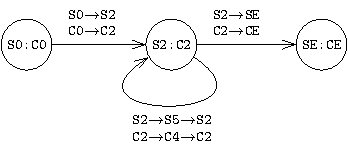
\includegraphics[scale=1.1]{chapters/figures/figSumListProductCfg.pdf}}
\end{center}
\caption{\label{fig:llTraverseProduct}Product-CFG}
\end{subfigure}%
&
\begin{subfigure}[b]{0.55\textwidth}
\begin{center}
\begin{footnotesize}
\begin{tabular}{|c|l|}
\hline
{\bf PC-Pair} & \multicolumn{1}{c|} {\bf Invariants} \\
\hline
\hline
(\scpc{0}{0}) &
\Tstrut $\circled{P}\  \sv{l} \indEq{} \lifted{list}{\mem{}}{lnode}{\cv{l}}$ \\
\multirow{2}{*}{(\scpc{2}{2})} &
\Tstrut $\circled{\scriptsize I1}\  \sv{l} \indEq{} \lifted{list}{\mem{}}{lnode}{\cv{l}}$ \\ &
\Tstrut $\circled{\scriptsize I2}\  \sv{sum} = \cv{sum}$ \\
(\scpc{E}{E}) &
\Tstrut $\circled{\scriptsize E}\  \sv{ret} = \cv{ret}$ \\
\hline
\end{tabular}
\end{footnotesize}
\vspace{13px}
\end{center}
\caption{\label{fig:llTraverseProductInv}Node Invariants of the Product-CFG}
\end{subfigure}%
\\
\end{tabular}
\caption{\label{fig:llTraverseProductCFGInvs} Product-CFG between the IRs in \cref{fig:llTraverseSpecIR,fig:llTraverseCIR}. The inductive invariants of the Product-CFG are given in \cref{fig:llTraverseProductInv}.}
\end{figure}


\subsection{Handling Type II Proof Obligations}
\label{sec:syn-cat2}
Consider the pair of programs in \cref{fig:llTraverseSpecIR,fig:llTraverseCIR}
that traverse a list to compute the sum of all elements.
The corresponding product-CFG and its node
invariants that ensure observable
equivalence are shown in \cref{fig:llTraverseProduct,fig:llTraverseProductInv}.

Consider the proof obligation originating due to \circled{\small I2} invariant across edge \scedge{2}{2}{2}{2} in \cref{fig:llTraverseProduct}:
\hoareTriple{\scpcinv{2}{2}}{\spath{2,5,2}, \cpath{2,4,2}}{\sv{sum} = \cv{sum}}, where
the node invariant \scpc{2}{2} contains the \recursiveRelation{} $\sv{l} \indEq{} \lifted{list}{\mem{}}{lnode}{\cv{l}}$.
The corresponding (simplified) first-order logic formula for this proof obligation is:
$(\sv{l} \indEq \lifted{list}{\mem{}}{lnode}{\cv{l}} \land \sv{sum} = \cv{sum} \land \neg(\sumIs{\sv{l}}{LNil}) \land \cv{l}\neq0) \Rightarrow (\sv{sum} + \prodAccess{\sv{l}}{val}) = (\cv{sum} + \structPointer{\cv{l}}{\mem{}}{lnode}{val})$.
We fail to remove the \recursiveRelation{} on the \lhs{} even after
$k$-unrolling for any finite unrolling parameter $k$ because both sides of \indEq{}
represent list values of arbitrary length.
In such a scenario, we do not know of an efficient
SMT encoding for the \recursiveRelation{} $\sv{l} \indEq{} \lifted{list}{\mem{}}{lnode}{\cv{l}}$.
Ignoring this \recursiveRelation{} will incorrectly (although soundly) evaluate
the proof obligation to false; however, for a successful equivalence
proof, we need the proof discharge algorithm to evaluate it to true. Let's call this
requirement \circled{\footnotesize R1}.

Now, consider the proof obligation formed by correlating two iterations
of the loop in program $S$ with one iteration of the loop in program $C$:
\hoareTriple{\scpcinv{2}{2}}{\spath{2,5,2,5,2}, \cpath{2,4,2}}{\sv{sum} = \cv{sum}}.
Similar to the last proof obligation, its equivalent first-order logic formula contains a \recursiveRelation{} in the \lhs{}.
Clearly, this proof obligation should evaluate to false.
% The equivalent
% first-order logic formula is:
% ($l_{S}\indEq{}Clist^{{\tt lnode}}_{m}(l_{C}) \land {\tt sum}_S={\tt sum}_C \land \neg({\tt l_S}\ is\ {\tt LNil}) \land \neg({\tt l_S.tail}\ is\ {\tt LNil})) \Rightarrow (({\tt sum}_S + l_S.val + l_S.tail.val) = (sum_C + \structPointer{l}{m}{{\tt lnode}}{val}))$.  After one unrolling
% of $l_{S}\indEq{}Clist^{{\tt lnode}}_{m}(l_{C})$,
% this proof obligation evaluates to false.
Whenever a proof obligation evaluates to false, we
expect an ideal proof discharge algorithm to generate a
counterexample that falsifies the proof obligation.
Let's call this requirement \circled{\footnotesize R2}.
Recall that these counterexamples help in faster
convergence of our invariant inference and correlation algorithms.

To tackle requirements \circled{\footnotesize R1} and \circled{\footnotesize R2},
our proof discharge algorithm converts the original proof obligation $P: \hoareTriple{\phi_s}{e}{\phi_d}$
into two approximated proof obligations $(P_{pre-o}: \hoareTriple{\phi^{o_{d_1}}_s}{e}{\phi_d})$
and $(P_{pre-u}: \hoareTriple{\phi^{u_{d_2}}_s}{e}{\phi_d})$.
Here $\phi^{o_{d_1}}_s$ and $\phi^{u_{d_2}}_s$ represent the over- and under-approximated
versions of precondition $\phi_s$ respectively, and $d_1$ and $d_2$ represent
{\em depth parameters} that indicate the degree of over- and
under-approximation. We over (under) approximate a predicate by over (under)
approximating each of its constituent \recursiveRelation{}.
The $d$-depth over- and under-approximations of a \recursiveRelation{} $l_1\indEq{}l_2$
are written as $l_1\indEqDepth{d}l_2$ and $l_1\indEqUapprox{d}l_2$ respectively.
To define these two operators, we start with the notion of {\em depth of an ADT value}.
The {\em depth} of an ADT value is simply the depth in its expression tree representation.
We also assign a depth to each node in the said representation.
The depth of the root node is defined to be zero.
For example, the \type{List} value \cons{LCons}(2, \cons{LCons}(4, \cons{LNil})) has a depth of 2.


$l_1\indEqDepth{d}l_2$ asserts equality of the corresponding structures and scalar values (i.e. boolean and bitvector values)
up to a depth of $d$. $l_1\indEqUapprox{d}l_2$ asserts equality of the corresponding structures
and scalar values up to a depth of $d$ and bounds the depths of $l_1$ and $l_2$ to a maximum of $d$.
$l_1\indEqUapprox{d}l_2$ is equivalent to $l_1\indEqDepth{d}l_2 \land \depthBound{d}{l_1} \land \depthBound{d}{l_2}$,
where $\depthBound{d}{l}$ asserts that $l$ has a maximum depth of $d$.
Unlike \recursiveRelations{}, these operators only equate
scalar expressions and can be encoded in SMT logic.
For example, the condition $l \indEqDepth{1} \lifted{list}{\mem{}}{lnode}{p}$
reduces to the SMT-encodable predicate:
$(\sumIs{l}{LNil} = (p = 0)) \land (\neg(\sumIs{l}{LNil}) \rightarrow (\prodAccess{l}{val} = \structPointer{p}{\mem{}}{lnode}{val}))$.
Similarly, $\depthBound{2}{l}$ is equivalent to
$(\sumIs{l}{LNil}) \vee (\neg(\sumIs{l}{LNil}) \land (\sumIs{\prodAccess{l}{tail}}{LNil}))$
and $\depthBound{2}{\lifted{list}{\mem{}}{lnode}{p}}$ is equivalent to
$(p = 0) \vee ((p \neq 0) \land (\structPointer{p}{\mem{}}{lnode}{next} = 0))$.

Thus, for a {\em Type II} proof obligation $P: \hoareTriple{\phi_s}{e}{\phi_d}$,
we first submit the over-approximated proof obligation $P_{pre-o}$
and return true if it evaluates to true.
Otherwise, we submit the under-approximated proof obligation $P_{pre-u}$.
If it returns false, then we return false with the counterexample.
If both approximations fail, we soundly return false with no counterexamples.

Revisiting our proof obligations, \hoareTriple{\scpcinv{2}{2}}{\spath{2,5,2}, \cpath{2,4,2}}{\sv{sum} = \cv{sum}}
is provable using a depth-1 overapproximation of the precondition $\scpcinv{2}{2}$.
% The depth-1 overapproximation retains the
% information that the first value in lists ${\tt l}_S$
% and ${\tt l}_C$ are equal, and that is sufficient to prove that
% the new values of $sum_{S}$ and $sum_{C}$ are also equal (given that the
% old values are equal, as encoded in $\phi_{{\tt S2:C2}}$).
Similarly, the proof obligation
\hoareTriple{\scpcinv{2}{2}}{\spath{2,5,2,5,2}, \cpath{2,4,2}}{\sv{sum} = \cv{sum}}
evaluates to false (with a counterexample) using
a depth-2 underapproximation of the precondition $\scpcinv{2}{2}$.
The following is a possible counterexample for a depth-2 underapproximation.
% In the depth-2 underapproximate version, we try to prove that
% if the equal lists $l_S$ and ${\tt Clist}^{{\tt lnode}}_{m}(l_C)$
% have exactly two
% nodes\footnote{The underapproximation
% restricts both lists to have at most
% two nodes; the path condition for ${\tt S2\rightarrow S5\rightarrow S2\rightarrow S5\rightarrow S2}$ additionally
% restricts $l_S$ to have at least two nodes; together, this is equivalent to the list having
% exactly two nodes}, then
% the sum of the values in the two nodes of $l_S$ is equal to the
% value stored in the first node in {\tt l}$_C$.
% This proof obligation will return a counterexample that
% maps program variables to their concrete values. We show a
% possible counterexample to this proof obligation below.
%
% \begin{small}
% \begin{center}
% \begin{footnotesize}
% \begin{tabular}{cc|c}
% {\tt sum$_S$ $\mapsto$ 3} & {\tt sum$_C$ $\mapsto$ 3} & \multirow{3}{*}{
% $m$ $\mapsto$ $\Bigg($
% \begin{tabular}{l}
% {\tt 0x123} $\mapsto_{\tt lnode}$ (.value $\mapsto$ 42, .next $\mapsto$ {\tt 0x456}), \\
% {\tt 0x456} $\mapsto_{\tt lnode}$ (.value $\mapsto$ 43, .next $\mapsto$ {\tt 0x000}), \\
% () $\mapsto$ {\tt 77} \\
% \end{tabular}
% $\Bigg)$
% } \\
% \multicolumn{2}{l|}{{\tt l$_S$} $\mapsto$ {\tt LCons(42,LCons(43,LNil))}} \\
% \multicolumn{2}{l|}{{\tt l$_C$} $\mapsto$ {\tt 0x123}} \\
% \end{tabular}
% \end{footnotesize}
% \end{center}
% \end{small}
% \begin{center}
% \begin{footnotesize}
% \begin{tabular}{l@{ $\mapsto$ }l|l}
% {\tt sum$_S$} & {\tt 3} &
% \multirow{4}{*}{
% $m$ $\mapsto$ $\Bigg($
% \begin{tabular}{l}
% {\tt 0x123} $\mapsto_{\tt lnode}$ (.value $\mapsto$ 42, .next $\mapsto$ {\tt 0x456}), \\
% {\tt 0x456} $\mapsto_{\tt lnode}$ (.value $\mapsto$ 43, .next $\mapsto$ {\tt 0x000}), \\
% () $\mapsto$ {\tt 77} \\
% \end{tabular}
% $\Bigg)$
% }
% \\
% {\tt sum$_C$} & {\tt 3} \\
% ${\tt l}_S$   & {\tt LCons(42,LCons(43,LNil))} \\
% ${\tt l}_C$   & {\tt 0x123} \\
% \end{tabular}
% \end{footnotesize}
% \end{center}
\begin{small}
\begin{center}
\begin{tabular}{ll@{ $\mapsto$ }l}
\{ & \sv{sum} & {\tt 3},\\
   & \cv{sum} & {\tt 3},\\
   & \sv{l} & {\tt LCons(42,LCons(43,LNil))},\\
   & \cv{l} & {\tt 0x123},\\
   & \mem{} & $\Bigg\{$
           \begin{tabular}{ll}
             & {\tt 0x123} $ \mapsto_\type{lnode}$ (.\field{value} $\mapsto$ {\tt 42}, .\field{next} $\mapsto$ {\tt 0x456}),\\
              & {\tt 0x456} $\mapsto_\type{lnode}$ (.\field{value} $\mapsto$ {\tt 43}, .\field{next} $\mapsto$ {\tt 0}),\\
              & () $\mapsto$ {\tt 77}\\
           \end{tabular}$\Bigg\}$ \\
\}\\
\end{tabular}
\end{center}
\end{small}
% This counterexample maps variables to values (e.g., {\tt sum}$_C$ maps to an {\tt i32} value {\tt 3}
% and {\tt l}$_S$ maps to a {\tt List} value {\tt LCons(42,LCons(43,LNil))}).
% It also maps the C program's memory state $m$ to an array that
% maps the regions starting at addresses {\tt 0x123} and {\tt 0x456} (regions of size
% `{\tt sizeof lnode}') to memory objects of type {\tt lnode} (with the
% {\tt value} and {\tt next} fields shown for each object). For all other addresses (except
% the ones for which an explicit mapping is available), $m$ maps them
% to the default byte-value {\tt 77} (shown
% as {\tt () $\mapsto$ 77}) in this counterexample.

% This counterexample satisfies the preconditions $l_S\indEqUapprox{2}{\tt Clist}^{{\tt lnode}}_{m}({\tt l}_C)$
% and $sum_S=sum_C$. Further, when the
% paths $({\tt S2\rightarrow S5\rightarrow S2\rightarrow S5\rightarrow S2}, {\tt C2\rightarrow C4\rightarrow C2})$
% are executed starting at the machine state represented by this counterexample, the resulting
% values of $sum_S$ and $sum_C$ are {\tt 3+42+43=88} and {\tt 3+42=45} respectively. Evidently, the
% counterexample falsifies the proof condition because these values are not equal (as required by the postcondition).

\subsection{Handling Type III Proof Obligations}
\label{sec:syn-cat3}
In \cref{fig:llAllocProductCFG}, consider a proof obligation generated
across the product-CFG edge \scedge{3}{5}{3}{3} while checking if the
\circled{\small I4} invariant, $\sv{l} \indEq{} \lifted{list}{\mem{}}{lnode}{\cv{l}}$, holds at (\scpc{3}{3}):
\hoareTriple{\scpcinv{3}{5}}{\spath{3,5,3}, \cpath{5,3}}{\sv{l} \indEq{} \lifted{list}{\mem{}}{lnode}{\cv{l}}}.
Here, a \recursiveRelation{} is present both in the precondition $\scpcinv{3}{5}$ (\circled{\small I8})
and in the postcondition (\circled{\small I4}) and we are unable to remove them after $k$-unrolling.
When lowered to first-order logic
through {\tt WP}$_{\spath{3,5,3}, \cpath{5,3}}$, this translates to (showing only relevant relations):
\begin{equation}
\begin{split}
\label{eqn:ex1cat3}
(\sv{i}=\cv{i} \land \cv{p}={\tt malloc()} \land \sv{l} \indEq{} \lifted{list}{\mem{}}{lnode}{\cv{l}}) \\ \Rightarrow (\cons{LCons}(\sv{i}, \sv{l}) \indEq{} \lifted{list}{\mem{}'}{lnode}{\cv{p}})
\end{split}
\end{equation}
On the \rhs{} of this first-order logic formula, $\cons{LCons}{\sv{i}, \sv{l}}$ is compared for
equality with $\lifted{list}{\mem{}'}{lnode}{\cv{p}}$; here \cv{p}
represents the address of the newly allocated \type{lnode} object (through {\tt malloc}) and $\mem{}'$
represents the C memory state after executing the writes at lines \cpc{5} and \cpc{6} on the path \cpath{5,3}, i.e.,
\begin{equation}
\label{eqn:memstore}
\mem{}' \equiv \mem[\& (\structPointer{\cv{p}}{\mem{}}{lnode}{val}) \leftarrow \cv{i}]_\type{i32}[\& (\structPointer{\cv{p}}{\mem{}}{lnode}{next}) \leftarrow \cv{l}]_\type{i32}
\end{equation}
Here, \memWrite{\mem{}}{a}{v}{T} represents an array that is
equal to \mem{} everywhere except at addresses starting at $a$ which contains the value $v$ of type \type{T}.
We also refer to these memory writes that distinguish \mem{} and $\mem{}'$, the {\em distinguishing writes}.

\subsubsection{LHS-to-RHS Substitution and RHS Decomposition}
We start by utilizing
the \indEq{} relationships in the \lhs{} (antecedent) of `$\Rightarrow$'
to rewrite \cref{eqn:ex1cat3} so that the ADT variables (e.g., \sv{l}) in its \rhs{} (consequent)
are substituted with the lifted $C$ values (e.g., \lifted{list}{\mem{}}{lnode}{\cv{l}}). Thus, we
rewrite \cref{eqn:ex1cat3} to:
%\begin{equation}\label{eqn:clistsEqualUnder}
%({\tt l}_S \indEq{} {\tt Clist}_m^{{\tt lnode}}({\tt l}_C)) \Rightarrow
%({\tt Clist}_m^{{\tt lnode}}({\tt l}_C) \indEq{} {\tt Clist}_{m'}^{{\tt lnode}}({\tt l}_C))
%\end{equation}
\begin{equation}
\label{eqn:ex2cat3}
\begin{split}
(\sv{i}=\cv{i} \land \cv{p}={\tt malloc()} \land \sv{l} \indEq{} \lifted{list}{\mem{}}{lnode}{\cv{l}}) \\ \Rightarrow (\cons{LCons}(\sv{i}, \lifted{list}{\mem{}}{lnode}{\cv{l}}) \indEq{} \lifted{list}{\mem{}'}{lnode}{\cv{p}})
\end{split}
\end{equation}
Next, we decompose the \rhs{} by decomposing the \recursiveRelation{} in the \rhs{}
followed by \rhs{}-breaking. This process reduces \cref{eqn:ex2cat3} into the following
smaller proof obligations (showing only the \rhs{}, the \lhs{} is the same as in \cref{eqn:ex2cat3}):
(a) $\neg(\cv{p} = 0)$,
(b) $\neg(\cv{p} = 0) \rightarrow (\sv{i} = \structPointer{\cv{p}}{\mem{}'}{lnode}{val})$, and
(c) $\neg(\cv{p} = 0) \rightarrow (\lifted{list}{\mem{}}{lnode}{\cv{l}} \indEq{} \lifted{list}{\mem{}'}{lnode}{\structPointer{\cv{p}}{\mem{}'}{lnode}{next}})$
The first two proof obligations fall in {\em Type II} and
are discharged through over- and under-approximation schemes (as discussed
in \cref{sec:syn-cat2}). Note that the first proof obligation is provable due
to the \cfits{} assumption which implies that pointer returned by {\tt malloc} must be non-null.
For ease of exposition, we simplify the postcondition of the third proof obligation
using the \cfits{} assumption and \cref{eqn:memstore} to:
% from
% {\small \tt $\neg({\tt p}_C=0)$ $\rightarrow$ (Clist$_{m}^{{\tt lnode}}$(l$_C$)$\indEq{}$Clist$_{m'}^{{\tt lnode}}$(p$_C\xrightarrow[]{m'}_{\mathrm{\tt lnode}}$next))}
% to
% {\tt (Clist$_{m}^{{\tt lnode}}$(l$_C$)$\indEq{}$Clist$_{m'}^{{\tt lnode}}$(l$_C$))}.
% This simplification is valid because {\tt l$_C$}
% is written
% to address {\tt \&(p$_C\xrightarrow[]{m'}_{\mathrm{\tt lnode}}$next)}
% in $m'$ (\cref{eqn:memstore}).
% Also, we have already
% shown that $\neg({\tt p}_C=0)$ holds.
% Thus, the third proof obligation can be rewritten as
% a \recursiveRelation{} between two lifted expressions:
\begin{equation}
\label{eqn:clistPreserved}
\lifted{list}{\mem{}}{lnode}{\cv{l}} \indEq{} \lifted{list}{\mem{}'}{lnode}{\cv{l}}
\end{equation}

Hence, we are interested in proving equality
between two \type{List} values in $C$ under different memory states \mem{} and $\mem{}'$.
%Note that in general this \recursiveRelation{} may be under an precondition.
Next, we show how the above can be posed as a bisimilarity check between
two programs.

% Thus,
% under an antecedent that ${\tt Clist}_m^{{\tt lnode}}({\tt l}_C)$
% is recursively equal to a {\tt List} value {\tt l}$_S$ in \SpecL{},
% we are interested in proving
% ${\tt Clist}_m^{{\tt lnode}}({\tt l}_C) \indEq{}
% {\tt Clist}_{m'}^{{\tt lnode}}({\tt l}_C)$.  We next show how this
% \recursiveRelation{} can be converted to a bisimulation proof.

%Informally, this proof obligation in \cref{eqn:clistPreserved} checks
%that the structure
%and values of the linked list pointed-to by {\tt l}$_C$
%in $m$ remain preserved even after the
%memory writes to the newly allocated node (in $m'$).
%At a minimum, such reasoning requires an alias analysis
%that confirms that the newly allocated node is isolated from
%the existing linked list nodes.  We discuss this in more
%detail in the following section.

\subsubsection{Equality of Values to Equivalence of Programs}
\label{sec:recursiveEqToBisim}
Consider a program that recursively calls the definition (body) of
\lift{list}{}{lnode} to deconstruct \lifted{list}{\mem{}}{lnode}{\cv{l}}.
For example, \lifted{list}{\mem{}}{lnode}{\cv{l}} may yield a recursive call
to \lifted{list}{\mem{}}{lnode}{\structPointer{\cv{l}}{\mem{}}{lnode}{next}}
and so on, until the argument becomes zero.
This program essentially deconstructs \lifted{list}{\mem{}}{lnode}{\cv{l}}
into its terminal (scalar) values and reconstructs
a \type{List} value equal to the value
represented by \lifted{list}{\mem{}}{lnode}{\cv{l}}.
We call this program a {\em deconstruction program} based
on the lifting constructor \lift{list}{}{lnode}.
% We call this program that deconstructs
% ${\tt Clist}_m^{{\tt lnode}}({\tt l}_C)$
% into its components and reconstructs an output
% {\tt List} value,
% a {\em reconstruction program} based on the unrolling procedure of
% ${\tt Clist}_m^{{\tt lnode}}({\tt l}_C)$.
%(using the unrolling procedure in \cref{eqn:clist}) until
%a null pointer is reached
%yields a sequence of
%${\tt Clist}_m^{{\tt lnode}}({\tt l}^0_C)$,
%${\tt Clist}_m^{{\tt lnode}}({\tt l}^1_C)$,
%${\tt Clist}_m^{{\tt lnode}}({\tt l}^2_C)$, ...
%values, where each
%{\tt l}$^i_C$ (for $i$=0,1,2,...)
%represents a C pointer in $m$ that is lifted
%to a {\tt List} value (using ${\tt Clist}_m^{{\tt lnode}}$)
%during this deconstruction. If this sequence is finite,
%its last value
%is {\tt LNil}.
%We call this series of C pointers
%${\tt l}^0_C$,
%${\tt l}^1_C$,
%${\tt l}^2_C$, ..., the {\tt Clist}$_m^{{\tt lnode}}$-reachable
%pointers of {\tt l}$^0_C$, or \Reachable{{\tt Clist}_m^{{\tt lnode}}}{${\tt l}^0_C$}.

%\begin{definition}
%A lifted ${\tt Clist}_m^{{\tt lnode}}({\tt l}_C))$ value
%is {\em well-formed} iff there exists a {\tt List} value ${\tt l}_S$
%in the \SpecL{} program $S$ such that
%$({\tt l}_S \indEq{} {\tt Clist}_m^{{\tt lnode}}({\tt l}_C))$.
%\end{definition}
%
%\begin{lemma}\label{lemma:finitenessOfWellFormed}
%For a well-formed lifted
%value ${\tt Clist}_m^{{\tt lnode}}({\tt l}_C))$,
%\Reachable{{\tt Clist}_m^{{\tt lnode}}}{${\tt l}^0_C$} is finite.
%\end{lemma}
%\begin{proof}
%\Cref{lemma:finitenessOfWellFormed} follows from the definition of well-formedness and the finiteness
%of any ADT value in the \SpecL{} language.
%\end{proof}
%
%\begin{theorem}\label{theorem:clistsEqual}
%For a well-formed lifted value ${\tt Clist}_m^{{\tt lnode}}({\tt l}_C))$:
%\begin{gather*}
%{\tt Clist}_m^{{\tt lnode}}({\tt l}_C)
%\indEq{}
%{\tt Clist}_{m'}^{{\tt lnode}}({\tt l}_C)\\
%\Leftrightarrow\\
%(\ReachableMath{{\tt Clist}_m^{{\tt lnode}}}{{\tt l}_C} = \ReachableMath{{\tt Clist}_{m'}^{{\tt lnode}}}{{\tt l}_C}\ \ \land\\
%\forall_{{{\tt l}^i_C\in\ReachableMath{{\tt Clist}_m^{{\tt lnode}}}{{\tt l}_C}}}({\structPointer{l^i_C}{m}{s}{value}}={\structPointer{l^i_C}{m'}{s}{value}} \land\ {\structPointer{l^i_C}{m}{s}{next}}={\structPointer{l^i_C}{m'}{s}{next}}))
%\end{gather*}
%\end{theorem}
%\begin{proof}
%The proof proceeds by induction on the structure of the
%well-formed value ${\tt Clist}_m^{{\tt lnode}}({\tt l}_C))$.
%The `{\tt l}$_C=0$' condition represents the base case.
%The induction step involves unifying the expansions of
%${\tt Clist}_m^{{\tt lnode}}$
%and
%${\tt Clist}_{m'}^{{\tt lnode}}$ obtained using \cref{eqn:clist}, and using the induction hypothesis.
%\end{proof}

% \begin{theorem}\label{theorem:clistsEqual}
% Under the antecedent
% $({\tt l}_S \indEq{} {\tt Clist}_m^{{\tt lnode}}({\tt l}_C))$:

% $({\tt Clist}_m^{{\tt lnode}}({\tt l}_C)
% \indEq{}
% {\tt Clist}_{m'}^{{\tt lnode}}({\tt l}_C))$
% holds iff a bisimulation relation
% exists between the reconstruction programs
% based on ${\tt Clist}_m^{{\tt lnode}}({\tt l}_C)$
% and
% ${\tt Clist}_{m'}^{{\tt lnode}}({\tt l}_C)$.
% The bisimulation relation must ensure that the
% observables generated by both procedures are
% identical.
% \end{theorem}
% \begin{proof}\let\qed\relax
% The ``if'' case of this ``iff'' relation follows
% from noting that the observables of
% a reconstruction program are the
% generated {\tt List} values. Thus, a
% successful bisimulation
% check ensures equal
% {\tt List}
% values upon termination. Termination
% follows from the antecedent because
% \SpecL{} values (such as $l_S$) must be finite.

% The ``only if'' case
% follows from the unification of the
% unrolling procedure (in \cref{eqn:clist}) for
% ${\tt Clist}_m^{{\tt lnode}}({\tt l}_C)$
% and
% ${\tt Clist}_{m'}^{{\tt lnode}}({\tt l}_C)$.

%The proof proceeds by induction on the structure of the
%${\tt Clist}_m^{{\tt lnode}}({\tt l}_C))$.
%The base case is
%represented by the `{\tt l}$_C=0$' condition ---
%both deconstruction procedures terminate in this case (irrespective
%of the contents of $m$ and $m'$).
%The induction step involves unifying the expansions of
%${\tt Clist}_m^{{\tt lnode}}$
%and
%${\tt Clist}_{m'}^{{\tt lnode}}$ obtained using \cref{eqn:clist}, and using the induction hypothesis.
%At the induction step, we need to show that the first procedure takes the \underline{if} branch
%iff the second procedure takes the \underline{if} branch.  Further, we need
%to show that whenever the {\tt value}
%and {\tt next} fields are read
%in the {\tt lnode} objects pointed-to by {\tt l$_C$} in $m$ and $m'$
%respectively, they have identical contents.
% \end{proof}

\begin{figure}[t]
\begin{tabular}{cc}
\begin{subfigure}[b]{0.49\textwidth}
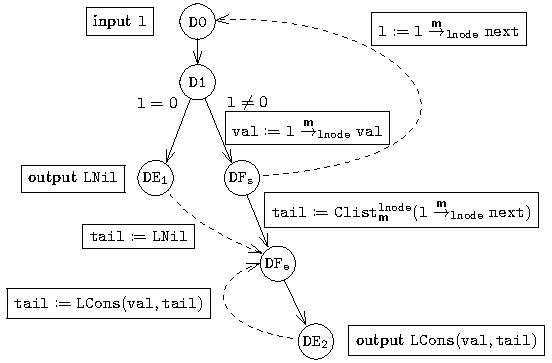
\includegraphics[scale=0.8]{chapters/figures/figClistCfg.pdf}
\vspace{3px}
\caption{\label{fig:reconsProg}Reconstruction Program}
\end{subfigure}%
&
\begin{subfigure}[b]{0.51\textwidth}
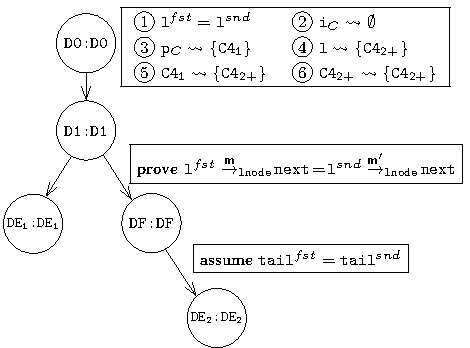
\includegraphics[scale=0.85]{chapters/figures/figClistProductCfg.pdf}
\vspace{17px}
\caption{\label{fig:reconsPCFG}Recons-PCFG}
\end{subfigure}%
%&
%\begin{subfigure}[b]{0.17\textwidth}
%\includegraphics[scale=0.8]{figMallocPointsToGraph.pdf}
%\caption{\label{xxx}XXX}
%\end{subfigure}%
\\
\end{tabular}
\caption{\label{fig:recons}Reconstruction program for \lifted{list}{\mem{}}{lnode}{l} and recons-PCFG between reconstruction programs of \lifted{list}{\mem{}}{lnode}{\cv{l}} and \lifted{list}{\mem{}'}{lnode}{\cv{l}} respectively. \\
In \cref{fig:reconsProg}, the square boxes show the transfer functions based on \cref{eqn:clist}.\\
The dashed edges represent a function call. In \cref{fig:reconsPCFG}, the square box to the \\ right of node (\rrpc{0}{0}) contains the inferred invariants for this recons-PCFG.}
\end{figure}


To check if $\lifted{list}{\mem{}}{lnode}{\cv{l}} \indEq{} \lifted{list}{\mem{}'}{lnode}{\cv{l}}$, we instead
check if a bisimulation relation exists
between the two respective deconstruction programs (assuming \lhs{} as the precondition at entries).
Similar to the top-level bisimulation search, we use a product-CFG to represent this bisimulation relation.
To distinguish this product-CFG from the top-level product-CFG that relates $S$ and $C$, we call
this product-CFG that relates two deconstruction programs, a {\em deconstruction product-CFG}
or {\em decons-PCFG} for short.
% To check bisimulation, we attempt to show that both reconstructions
% proceed in lockstep, and the invariants at
% each step of this lockstep execution ensure equal observables.
% We use a product-CFG to encode this lockstep execution --- to distinguish this
% product-CFG from the top-level product-CFG that relates $S$ and $C$, we call
% this product-CFG that relates two reconstruction programs, a {\em reconstruction product-CFG}
% or {\em decons-PCFG} for short.
% i.e., (1) the first deconstruction procedure evaluates
%an \underline{if} condition (e.g., {\tt l$_C$=0}) to true iff the second
%deconstruction procedure also evaluates the
%corresponding \underline{if} condition to true; and (2)
%the values observed by the first deconstruction procedure (e.g., {\tt lnode.value}
%which is used for constructing the observable {\tt List}) are identical to the
%ones observed by the second deconstruction procedure.
%As we have seen earlier, this lockstep execution can be encoded
%as a product-CFG: the invariants at the nodes of this product-CFG
%represent the conditions that must hold at the correlated
%PCs of this
%lockstep execution; for
%a successful bisimulation check, these invariants must ensure equal observables.
The deconstruction
program and the decons-PCFG for our \lift{list}{}{lnode} example are shown in \cref{fig:recons}.
We distinguish states between the first and second programs using superscripts: $fst$ and $snd$ respectively.
However, these are omitted in case the states are equal in both programs (e.g., \cv{p}).
Since both \lifted{list}{\mem{}}{lnode}{\cv{l}}
and \lifted{list}{\mem{}'}{lnode}{\cv{l}} use the same
lifting constructor \lift{list}{}{lnode}, the PC-transition correlations of both programs
are trivially obtained by unifying the program structures.
A node is created in the decons-PCFG that
encodes the correlation of the entries to both programs,
we call this node the {\em recursive-node} in the decons-PCFG (e.g., \rrpc{0}{0} in \cref{fig:reconsPCFG}).
A recursive call becomes a back-edge in the decons-PCFG that terminates at the recursive-node.
% A candidate invariant at the recursive-node is obtained by equating the pair of corresponding $l$
% variables across the first (superscripted with $fst$) and second (superscripted with $snd$) programs.
At the start of both deconstruction programs, $\fstv{l} = \sndv{l} = \cv{l}$ --- the same \cv{l} is passed to
both deconstruction programs, only the memory states \mem{} and $\mem{}'$ are different.
The bisimulation check thus involves checking that if the invariant $\fstv{l} = \sndv{l}$
holds at the recursive-node, then during one iteration of the static programs:
\vspace{-13px}
\begin{enumerate}
\setlength{\itemsep}{-3px}
\item The \underline{\tt if} condition $(\fstv{l} = 0)$ in the first program is equal to the corresponding
\underline{\tt if} condition $(\sndv{l} = 0)$ in the second program.
\item If the \underline{\tt if} condition evaluates to false in both programs, then
the observable values (that are used in the construction of the list) are equal: \\
$((\fstv{l} \neq 0) \land (\sndv{l} \neq 0)) \Rightarrow (\structPointer{\fstv{l}}{\mem{}}{lnode}{val} = \structPointer{\sndv{l}}{\mem{}'}{lnode}{val})$.
\item If the \underline{\tt if} condition evaluates to false in both programs, then
the invariant holds at the beginning of the programs invoked through the
recursive call. This involves checking equality of the arguments to the recursive call: \\
$((\fstv{l} \neq 0) \land (\sndv{l} \neq 0)) \Rightarrow (\structPointer{\fstv{l}}{\mem{}}{lnode}{next} = \structPointer{\sndv{l}}{\mem{}'}{lnode}{next})$.
\end{enumerate}
\vspace{-10px}
The first check succeeds due to the invariant $\fstv{l} = \sndv{l}$.
For the second and third checks, we additionally
need to reason that the memory objects
$\structPointer{\comv{l}}{\mem{}}{lnode}{val}$ and $\structPointer{\comv{l}}{\mem{}}{lnode}{next}$ cannot
alias with the writes (in $\mem{}'$ in \cref{eqn:memstore}) to the newly allocated objects
$\structPointer{\cv{p}}{\mem{}}{lnode}{val}$ and $\structPointer{\cv{p}}{\mem{}}{lnode}{next}$.
We capture this aliasing information by running an interprocedural allocation-site based points-to analysis on
the original $C$ program as well as the deconstruction programs being checked
for equivalence. Our points-to analysis also splits each allocation site region, say \mlr{C4} in \cref{fig:llAllocCIR}, into
two regions \mlrf{C4} and \mlrs{C4}, where \mlrf{C4} represents the region of the most recent allocation and \mlrs{C4}
represents the region of all other allocations through ${\tt malloc_{C4}}$ respectively.
We write $p \pointsTo{} \{\mlr{R_1}, \mlr{R_2}\}$ to represent the condition that value $p$ {\em may point to}
an object belonging to one of the region labels \mlr{R_1} or \mlr{R_2}
(but may not point to any object outside of \mlr{R_1} and \mlr{R_2}). We compute may-point-to information for
all program variables as well as the region labels themselves.
% For example, at the start of PC {\tt C7} in \cref{fig:llAllocCIR},
% {\tt i}$_C\pointsTo{}\emptyset$,
% {\tt n}$_C\pointsTo{}\{{\tt C4}_1\}$,
% and {\tt l}$_C\pointsTo{}\{{\tt C4}_{2+}\}$.
% Because the may-point-to analysis determines the
% sets of objects pointed-to by {\tt n}$_C$ and {\tt l}$_C$ to
% be disjoint ($\{{\tt C4_{1}}\}$ vs. $\{{\tt C4_{2+}}\}$), any
% memory accesses through {\tt n}$_C$ and {\tt l}$_C$
% cannot alias at {\tt C7} (for an access
% offset that is within the bounds of
% the allocation size `{\tt sizeof lnode}').
% Similarly, at PC {\tt C7}, we
% get
% ${\tt C4}_{1}\pointsTo{}\{{\tt C4}_{2+}\}$ and
% ${\tt C4}_{2+}\pointsTo{}\{{\tt C4}_{2+}\}$.
% The condition
% ${\tt C4}_{1}\pointsTo{}\{{\tt C4}_{2+}\}$
% holds because the {\tt next} pointer of the object
% pointed-to by ${\tt n}_C$ (which
% is a ${\tt C4}_1$ object) may point to
% a {\tt C4}$_{2+}$ object (e.g., object pointed-to
% by {\tt l}$_C$).
% Similarly, ${\tt C4}_{2+}\pointsTo{}\{{\tt C4}_{2+}\}$
% says that a pointer within a {\tt C4}$_{2+}$ object
% may point to a {\tt C4}$_{2+}$
% object (but not to a {\tt C4}$_1$ object).

% \subsubsection{Transferring points-to information to the decons-PCFG}
% \label{sec:pointsToAsInvariants}
% Recall that
% in \cref{sec:recursiveEqToBisim},
% we reduce a validity check of the condition
% ${\tt Clist}_m^{{\tt lnode}}({\tt l}_C)
% \indEq{} {\tt Clist}_{m'}^{{\tt lnode}}({\tt l}_C)$
% to a bisimulation check. Also, recall
% that we discharge the bisimulation check through the construction
% of a decons-PCFG that compares the unrolling procedure with itself (executing
% on memory states $m$ and $m'$).
% During this bisimulation check, we need to prove
% that for each execution
% of the unrolling procedure, $\structPointer{{\tt l}_C}{m}{\tt lnode}{\{val,next\}}$
% and $\structPointer{{\tt l}_C}{m'}{\tt lnode}{\{val,next\}}$\footnote{Here, we use the symbol {\tt l}$_C$ to
% refer to equal values {\tt l}$^{fst}_C$ and
% {\tt l}$^{snd}_C$.} are equal.
% To successfully discharge these proof obligations, it suffices
% to show ${\tt l}_C$ cannot alias with the memory writes that
% distinguish $m$ from $m'$.
\vspace{-5px}
Our points-to analysis on
the C program determines that at PC \cpc{5} of \cref{fig:llAllocCIR} (the start of
the product-CFG edge \scedge{3}{5}{3}{3} across which the proof
condition is being evaluated), the pointer to the {\em head}
of the list, i.e., $\cv{l} \pointsTo{} \{ \mlrs{C4} \}$.
It also determines that the distinguishing
writes modify memory regions belonging to \mlrf{C4} only.
Further, we get $\mlrs{C4} \pointsTo{} \{ \mlrs{C4} \}$ at PC \cpc{5}.
However, notice that these determinations only rule out aliasing of the list-head with
the distinguishing writes. We also need to confirm non-aliasing
of the internal nodes of the linked list with the distinguishing writes.
For this, we need to identify a points-to invariant,
$\sndv{l} \pointsTo{} \{ \mlrs{C4} \}$, at the recursive-node
of the decons-PCFG (shown in \cref{fig:reconsPCFG}).
To identify such points-to invariant, we run our points-to analysis
on the deconstruction programs (\cref{fig:reconsProg}) before comparing them for equivalence.
To model procedure calls, a {\em supergraph} is created with control flow to and from the entry and exit
of the program (e.g., dashed edges in \cref{fig:recons}).
We use the results of the points-to analysis on $C$ at the PC where the proof obligation
is being discharged (\cpc{5} of \cref{fig:llAllocC} in our case).
To see why $\sndv{l} \pointsTo{} \{ \mlrs{C4} \}$ is
an inductive invariant at the recursive-node:
(base case) the invariant holds at entry to the decons-PCFG since it holds for \cv{l} and
(induction step) if $\sndv{l} \pointsTo{} \{ \mlrs{C4} \}$ holds at the entry node,
it also holds at the start of a recursive call.
This follows from $\mlrs{C4} \pointsTo{} \{ \mlrs{C4} \}$ (points-to information at PC \cpc{5}),
which ensures that $\structPointer{\cv{l}}{\mem{}'}{lnode}{next}$ may point to only \mlrs{C4} objects.
% \vspace{-10px}
% \begin{itemize}
% \setlength{\itemsep}{0px}  
% \item (Base case) The invariant holds
% at entry to the decons-PCFG (because it holds for ${\tt l}^{start}_C$).
% \item (Induction step) If ${\tt l}_C^{snd}\pointsTo{}\{{\tt C4}_{2+}\}$
% holds at the entry node,
% it also holds at the start of a recursive call. This
% follows from ${\tt C4}_{2+}\pointsTo{}\{{\tt C4}_{2+}\}$ (points-to information at PC {\tt C5}),
% which ensures that $\structPointer{\tt l_C}{m'}{\tt lnode}{next}$ may point to only ${\tt C4}_{2+}$ objects.
% \end{itemize}
% \vspace{-10px}
During proof obligation discharge (e.g., during the bisimulation check on decons-PCFG),
the points-to invariants are encoded as SMT constraints.
This allows us to successfully complete the bisimulation proof on the decons-PCFG, and
consequently successfully discharge the proof obligation
\hoareTriple{\scpcinv{3}{5}} {\spath{3,5,3}, \cpath{5,3}}{\sv{l} \indEq{} \lifted{list}{\mem{}}{lnode}{\cv{l}}}
generated due to \circled{\small I4} invariant in \cref{tab:llproductInv}.
% The points-to analysis is described more formally
% in \cref{sec:pointsToFormal}.
\vspace{-10px}
\subsection{Summary of Proof Discharge Algorithm}
\vspace{-5px}
\label{sec:syn-algosummary}
Let $Solve(\lhs{}, \rhs{}, k, d_o, d_u)$ be the top-level procedure for discharging proof obligations.
$\lhs{} \Rightarrow \rhs{}$ represents the proof obligation, where $k$, $d_o$ and $d_u$ are the categorization parameter,
over- and under-approximation depths respectively.
$Solve$ returns either {\tt T} or {\tt F}($\Gamma$) signifying proven and disproven respectively
where $\Gamma$ is a set of counterexamples.
We perform \rhs{}-breaking on the lowered proof obligations and invoke $Solve$ for each smaller proof obligations.
\Cref{algo:proofSummary} gives a broad overview of our proof discharge algorithm.

\begin{figure}[H]
\begin{algorithm}[H]
\begin{scriptsize}
\SetAlgoLined
\SetKwProg{Fn}{Function}{}{end}
\Fn{$Solve(\lhs{}, \rhs{}, k, d_o, d_u)$}{
  $(\lhs{}_k, \rhs{}_k) \mapsfrom DecomposeAndUnroll(\lhs{}, \rhs{}, k)$;\\
  \Switch{$Categorize(\lhs{}_k, \rhs{}_k)$}{
    \lCase{${\tt Type\ I}$}{\Return{$SMTSolve(\lhs{}_k \Rightarrow \rhs{}_k)$}}
    \uCase{${\tt Type\ II}$}{
      $(\lhs{}_o, \lhs{}_u) \mapsfrom Approximate(\lhs{}, d_o, d_u)$;\\
      \lIf{$SMTSolve(\lhs{}_o \Rightarrow \rhs{}_k) \equiv {\tt T}$}{\Return{${\tt T}$}}
      \lIf{$SMTSolve(\lhs{}_u \Rightarrow \rhs{}_k) \equiv {\tt F}(\Gamma)$}{\Return{${\tt F}(\Gamma)$}}
      \lElse{\Return{${\tt F}(\emptyset)$}}
    }
    \Case{${\tt Type\ III}$}{
      \ForEach{${\tt P}_i \Rightarrow \rhs{}_i : DecomposeAndRHSBreak(\lhs{}, \rhs{})$}{
        \uIf{$\rhs{}_i\ \equiv\ l_1\indEq{}l_2$}{
          $(D_1,D_2) \mapsfrom GetDeconstructionPrograms(l_1,l_2)$;\\
          \lIf{$CheckBisimilarity(\lhs{} \land {\tt P}_i,D_1,D_2) \equiv {\tt F}$}{\Return{${\tt F}(\emptyset)$}}
        }
        \Else{
          \lIf{$Solve(\lhs{} \land {\tt P}_i, \rhs{}_i, k, d_o, d_u) \equiv {\tt F}(\Gamma)$}{\Return{${\tt F}(\Gamma)$}}
        }
      }
      \Return{${\tt T}$};
    }
  }
}
\end{scriptsize}
\end{algorithm}
\caption{\label{algo:proofSummary} Summary of the Proof Discharge Algorithm}
\end{figure}

%Thus, as a part of the invariant inference procedure on the product-CFG
%for the decomposition programs, we also run our points-to analysis on the
%product-CFG to identify points-to invariants at the product-CFG
%nodes.  This improves precision, as shown in the example discussed
%above.
% \vspace{-5px}
% \subsubsection{Proof discharge algorithm for Type III obligations}
% \label{sec:cat3summary}

% Before the start of an equivalence check, a points-to analysis is run on the $C$ IR once.
% During the equivalence check,
% to discharge a Type III proof obligation $P: {\tt LHS}\Rightarrow{\tt RHS}$ (expressed
% in first-order logic), we first replace the recursive
% values of program $S$ in the {\tt RHS}
% with lifted C values, based on the equalities present in the {\tt LHS}, to
% obtain $P_2$.
% This is followed by decomposition and RHS-breaking of $P_2$.

% Upon successful decomposition, we
% obtain several smaller proof obligations.
% To prove $P$, we require all these smaller proof
% obligations to be provable. If any of these smaller proof obligations
% is not provable, we are unable to prove $P$.  If we obtain a counterexample
% to any of these smaller proof obligations, then that counterexample
% also falsifies $P$.
% Let $P_3$ represent any such smaller proof obligation.
% {\tt RHS} of $P_3$, being
% a decomposition clause,
% must relate atomic expressions on the {\tt RHS}.
% If $P_3$ relates two scalar values in the {\tt RHS}, then
% it is a Type II proof obligation and can be discharged
% using the algorithm in \cref{sec:cat2algo}.

% If $P_3$ relates two lifted
% expressions in
% the {\tt RHS},
% we check if the reconstruction
% programs of the two lifted ADT values being
% compared can be proven to be bisimilar (assuming that
% {\tt LHS} of $P_3$ holds at the correlated entry nodes
% in the decons-PCFG).
% To improve
% the bisimulation
% check's precision, we transfer the points-to information of the $C$ program
% (at the PC where the proof obligation is being discharged) to the entry
% of the reconstruction programs. The same points-to analysis is ran on the
% reconstruction programs to populate the points-to function at all PCs.

% These queries
% generated by a bisimulation check are discharged
% by a recursive call to the proof discharge procedure.
% The depth of these recursive calls to the
% proof discharge procedure is determined by
% the maximum {\em recursion nest depth} (similar
% to loop nest depth) of the decomposition
% program.

% If the bisimilarity check succeeds, the proof procedure returns
% true for $P$.
% If the bisimilarity check fails,
% we imprecisely return false for $P$ (without a counterexample).

% Finally, if $P_3$ neither
% relates two scalar values, nor relates two lifted expressions,
% we attempt to prove that {\tt LHS} of $P_3$ imply {\tt false}.
% If successfully disproven, we return false for $P$ with the counterexamples.
% Otherwise, we imprecisely return false for $P$ (without a counterexample).

% Please refer to {\tt Chapter \ThesisChapterAlgo{}} of the thesis for a
% detailed discussion on the algorithms introduced in this section along
% with their pseudo-code.